\documentclass[border=6pt]{standalone}
\usepackage{amsmath,amssymb,tikz,adjustbox}
\usetikzlibrary{arrows.meta,positioning,calc}
\begin{document}
\begin{adjustbox}{max width=440pt}
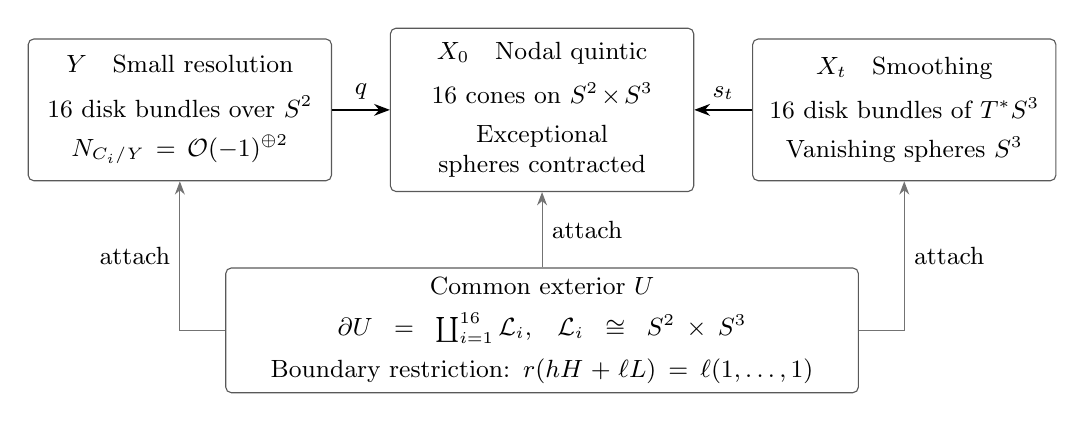
\begin{tikzpicture}[font=\small,>=Stealth,
 fibre/.style={draw=black!65,rounded corners=2pt,align=center,
 text width=3.5cm,minimum height=1.8cm,inner sep=5pt},
 map/.style={->,semithick},inc/.style={->,draw=black!55}]
\node[fibre] (Y) at (-4.6,0) {$Y$\quad Small resolution\\[5pt]
 $16$ disk bundles over $S^2$\\[3pt]
 $N_{C_i/Y}=\mathcal O(-1)^{\oplus2}$};
\node[fibre] (X) at (0,0) {$X_0$\quad Nodal quintic\\[5pt]
 $16$ cones on $S^2\!\times\! S^3$\\[3pt]
 Exceptional spheres contracted};
\node[fibre] (T) at (4.6,0) {$X_t$\quad Smoothing\\[5pt]
 $16$ disk bundles of $T^*S^3$\\[3pt]
 Vanishing spheres $S^3$};
\draw[map] (Y.east) -- node[above] {$q$} (X.west);
\draw[map] (T.west) -- node[above] {$s_t$} (X.east);
\node[draw=black!65,rounded corners=2pt,align=center,text width=7.8cm,
 minimum height=1.4cm] (U) at (0,-2.8)
 {Common exterior $U$\\[4pt]
 $\partial U=\coprod_{i=1}^{16}\mathcal L_i$,\quad
 $\mathcal L_i\cong S^2\times S^3$\\[4pt]
 Boundary restriction: $r(hH+\ell L)=\ell(1,\ldots,1)$};
\draw[inc] (U.west) -| node[pos=0.75,left] {attach} (Y.south);
\draw[inc] (U.north) -- node[right] {attach} (X.south);
\draw[inc] (U.east) -| node[pos=0.75,right] {attach} (T.south);
\end{tikzpicture}
\end{adjustbox}
\end{document}
